\documentclass[border=10pt]{standalone}
\usepackage{tikz}
\usetikzlibrary{arrows.meta,positioning}
\usepackage[T1]{fontenc}
\usepackage{lmodern}

\definecolor{nb}{HTML}{3D4574}
\definecolor{rb}{HTML}{B83232}
\definecolor{gb}{HTML}{27AE60}
\definecolor{sub}{HTML}{D4D8EA}
\definecolor{arenagreen}{HTML}{27AE60}

\tikzset{
  fbox/.style={
    rectangle, rounded corners=5pt, draw=none, fill=nb,
    text=white, font=\bfseries\large,
    minimum height=1.55cm, minimum width=7.2cm, text width=7.0cm,
    align=center, inner sep=8pt
  },
  rbox/.style={fbox, fill=rb},
  gbox/.style={fbox, fill=gb},
  tile/.style={
    rectangle, draw=nb!50!white, line width=0.8pt,
    fill=nb, text=white, font=\bfseries\normalsize,
    minimum width=1.55cm, minimum height=1.55cm, align=center
  },
  arr/.style={-Stealth, line width=1.8pt, black}
}

\begin{document}
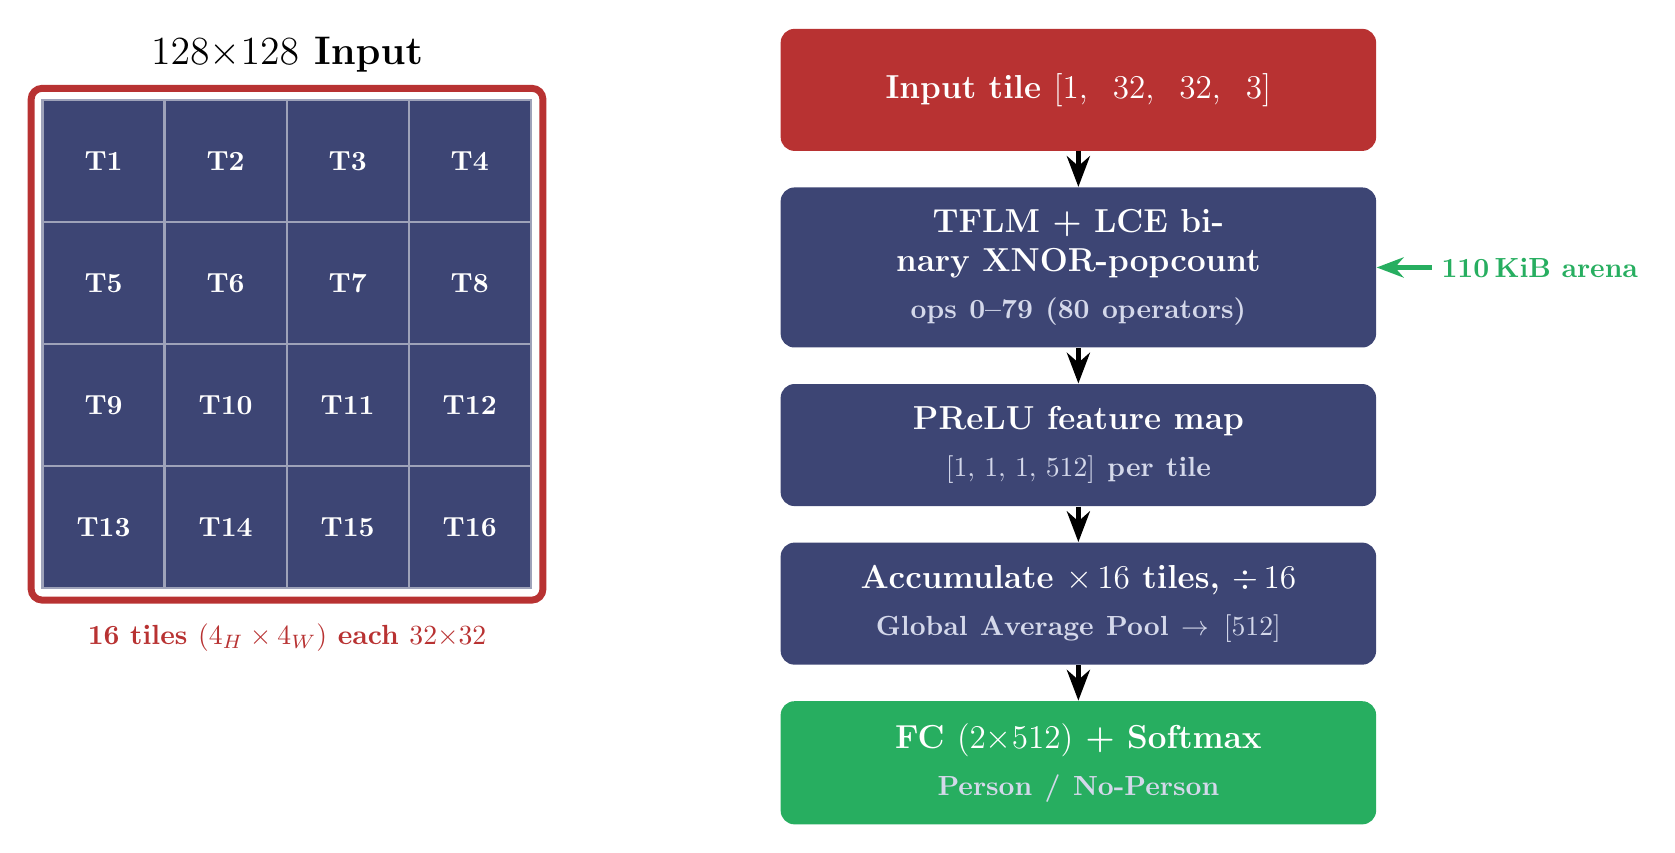
\begin{tikzpicture}

% ── Title ─────────────────────────────────────────────────────────
\node[font=\bfseries\Large, text=black] at (3.45, 0.35)
  {$128{\times}128$ Input};

% ── Red border: tight around tiles with 0.15 cm padding ───────────
% Tile x: [0.345, 6.545]  Tile y: [-0.225, -6.425]
\draw[rb, line width=2.5pt, rounded corners=4pt]
  (0.20, -0.08) rectangle (6.70, -6.58);

% ── Tile grid ─────────────────────────────────────────────────────
\foreach \row in {1,...,4}{
  \foreach \col in {0,...,3}{
    \pgfmathtruncatemacro{\n}{(\row-1)*4+\col+1}
    \node[tile] at ({1.55*\col + 1.12}, {-1.55*(\row-1) - 1.0})
      {T\n};
  }
}

% ── Grid caption ──────────────────────────────────────────────────
\node[rb, font=\normalsize\bfseries, text=rb] at (3.45,-7.05)
  {16 tiles $(4_H \times 4_W)$ each $32{\times}32$};

% ── Right: inference flow (positioned to the right of grid) ───────
\node[rbox] (inp) at (13.5, -0.1)
  {Input tile $[1,\;32,\;32,\;3]$};

\node[fbox, below=0.45cm of inp] (tflm)
  {TFLM + LCE binary XNOR-popcount
   \\[3pt]\textcolor{sub}{\normalsize ops 0--79 (80 operators)}};

\node[fbox, below=0.45cm of tflm] (feat)
  {PReLU feature map
   \\[3pt]\textcolor{sub}{\normalsize $[1,\,1,\,1,\,512]$ per tile}};

\node[fbox, below=0.45cm of feat] (acc)
  {Accumulate $\times\,16$ tiles, $\div\,16$
   \\[3pt]\textcolor{sub}{\normalsize Global Average Pool $\to [512]$}};

\node[gbox, below=0.45cm of acc] (fc)
  {FC $(2{\times}512)$ + Softmax
   \\[3pt]\textcolor{sub}{\normalsize Person / No-Person}};

% ── Arena label: clearly to the RIGHT of tflm ─────────────────────
\node[arenagreen, font=\bfseries\normalsize, anchor=west]
  (arenlbl) at ([xshift=0.7cm]tflm.east)
  {110\,KiB arena};
\draw[arenagreen, line width=1.5pt, -Stealth]
  (arenlbl.west) -- (tflm.east);

% ── Flow arrows ────────────────────────────────────────────────────
\draw[arr] (inp)  -- (tflm);
\draw[arr] (tflm) -- (feat);
\draw[arr] (feat) -- (acc);
\draw[arr] (acc)  -- (fc);

\end{tikzpicture}
\end{document}
